% ─────────────────────────────────────────────────────────────────────────────
% Informe: Modelamiento de la Ley de Mersenne mediante Regresión Simbólica
% Compilar con pdfLaTeX (compatible Overleaf)
% ─────────────────────────────────────────────────────────────────────────────
\documentclass[12pt,a4paper]{article}

% ── Codificación y lenguaje ───────────────────────────────────────────────────
\usepackage[utf8]{inputenc}
\usepackage[T1]{fontenc}
\usepackage[spanish,es-nodecimaldot]{babel}

% ── Matemáticas ───────────────────────────────────────────────────────────────
\usepackage{amsmath,amssymb,amsfonts}
\usepackage{mathtools}

% ── Física y unidades ─────────────────────────────────────────────────────────
\usepackage{siunitx}
\sisetup{output-decimal-marker={.}, separate-uncertainty=true}

% ── Diseño de página ──────────────────────────────────────────────────────────
\usepackage[top=2.5cm,bottom=2.5cm,left=2.8cm,right=2.8cm]{geometry}
\usepackage{setspace}
\onehalfspacing

% ── Figuras ───────────────────────────────────────────────────────────────────
\usepackage{graphicx}
\usepackage{subcaption}
\usepackage{float}
\graphicspath{{figurastex/}}

% ── Tablas ────────────────────────────────────────────────────────────────────
\usepackage{booktabs}
\usepackage{array}
\usepackage{multirow}
\usepackage{xcolor}
\usepackage{colortbl}

% ── Código ────────────────────────────────────────────────────────────────────
\usepackage{listings}
\lstset{
  basicstyle=\small\ttfamily,
  keywordstyle=\color{blue!70!black}\bfseries,
  commentstyle=\color{gray}\itshape,
  stringstyle=\color{orange!80!black},
  numbers=left, numberstyle=\tiny\color{gray},
  frame=single, rulecolor=\color{gray!40},
  backgroundcolor=\color{gray!5},
  breaklines=true, breakatwhitespace=true,
  tabsize=4, showstringspaces=false,
  language=Python,
}

% ── Diagramas TikZ ────────────────────────────────────────────────────────────
\usepackage{tikz}
\usetikzlibrary{arrows.meta,calc,decorations.pathmorse,decorations.pathreplacing}

% ── Hipervínculos ─────────────────────────────────────────────────────────────
\usepackage[colorlinks=true,linkcolor=blue!60!black,citecolor=green!50!black,
            urlcolor=blue!50!black]{hyperref}

% ── Cabecera / pie ────────────────────────────────────────────────────────────
\usepackage{fancyhdr}
\pagestyle{fancy}
\fancyhf{}
\fancyhead[L]{\small Ley de Mersenne — Regresión Simbólica}
\fancyhead[R]{\small \thepage}
\renewcommand{\headrulewidth}{0.4pt}

% ── Secciones con color ───────────────────────────────────────────────────────
\usepackage{titlesec}
\titleformat{\section}{\large\bfseries\color{blue!70!black}}{§\thesection.}{0.5em}{}[\titlerule]
\titleformat{\subsection}{\normalsize\bfseries\color{blue!40!black}}{\thesubsection.}{0.4em}{}

% ── Cajas de resultados ───────────────────────────────────────────────────────
\usepackage{tcolorbox}
\tcbuselibrary{skins,breakable}
\newtcolorbox{resultbox}[1][]{
  enhanced, breakable,
  colback=blue!4!white, colframe=blue!50!black,
  fonttitle=\bfseries, title=#1,
  left=4pt, right=4pt, top=4pt, bottom=4pt,
}
\newtcolorbox{warningbox}[1][]{
  enhanced,
  colback=orange!8!white, colframe=orange!70!black,
  fonttitle=\bfseries\color{orange!80!black}, title=#1,
  left=4pt, right=4pt,
}
\newtcolorbox{mersennebox}{
  enhanced, breakable,
  colback=green!5!white, colframe=green!50!black,
  fonttitle=\bfseries\color{green!40!black},
  title={Ley de Mersenne — Resultado principal},
  left=6pt, right=6pt, top=6pt, bottom=6pt,
}

% ─────────────────────────────────────────────────────────────────────────────
\begin{document}
% ─────────────────────────────────────────────────────────────────────────────

\begin{titlepage}
  \centering
  \vspace*{1.5cm}
  {\LARGE\bfseries\color{blue!70!black}
    Modelamiento de la Ley de Mersenne en una Guitarra Acústica\\[0.4em]
    mediante Regresión Simbólica
  }\par
  \vspace{1.2cm}
  {\large\itshape
    Construcción de un \emph{dataset} experimental bivariado\\
    y redescubrimiento de la fórmula $f_0 = \dfrac{1}{2L}\sqrt{\dfrac{T}{\mu}}$
  }\par
  \vspace{1.5cm}
  \rule{0.6\textwidth}{0.6pt}\\[0.8cm]
  {\large Juan Diego Montoya}\par
  \vspace{0.4cm}
  {\normalsize Modelamiento en Física Computacional}\par
  \vspace{0.3cm}
  {\normalsize\color{gray} Abril, 2026}\par
  \vspace{2cm}
  \begin{abstract}
    \noindent
    Se presenta el proceso completo de modelamiento de la \textbf{Ley de
    Mersenne} para cuerdas vibrantes utilizando datos obtenidos
    experimentalmente en una guitarra acústica D'Addario EJ16.
    Se extrajeron frecuencias fundamentales $f_0$ mediante la
    Transformada Rápida de Fourier (FFT) en 120 grabaciones de audio
    (6 cuerdas $\times$ 20 trastes). A continuación, cada variable de la
    ley de Mersenne fue estudiada de forma \emph{estrictamente
    bivariada}: $f_0(L)$ con ajuste potencial log-log, $f_0(\mu)$
    aprovechando la variedad de cuerdas del juego, y $f_0(T)$ mediante
    medición experimental de tensión con un diagrama de cuerpo libre.
    Finalmente, se aplicó regresión simbólica (log-lineal multivariable
    más búsqueda genética con \texttt{gplearn}) sobre el \emph{dataset}
    combinado. Los exponentes recuperados
    $b_L = -0.999$, $b_\mu = -0.473$, $b_T = +0.441$
    convergen hacia los valores teóricos de Mersenne
    $(-1,\,-\tfrac{1}{2},\,+\tfrac{1}{2})$ con un coeficiente de
    determinación $R^2 = 0.992$ en el modelo conjunto.
  \end{abstract}
\end{titlepage}

\tableofcontents
\newpage

% ═════════════════════════════════════════════════════════════════════════════
\section{Introducción}
% ═════════════════════════════════════════════════════════════════════════════

La \textbf{regresión simbólica} es una técnica de aprendizaje automático
que busca la forma funcional de una ley física directamente a partir de
datos, sin hipótesis previas sobre la expresión matemática. A diferencia
de la regresión paramétrica clásica, el algoritmo no ajusta parámetros de
un modelo ya fijado, sino que explora un espacio de expresiones generadas
por operaciones elementales (multiplicación, división, raíz, potencia, etc.)
mediante estrategias evolutivas.

En este trabajo se aplica esta metodología para \emph{redescubrir} la
\textbf{Ley de Mersenne}:
\begin{equation}
  \boxed{f_0 = \frac{1}{2L}\sqrt{\frac{T}{\mu}}}
  \label{eq:mersenne}
\end{equation}
donde $f_0$ es la frecuencia fundamental de la cuerda, $L$ la longitud
vibrante, $T$ la tensión y $\mu$ la densidad lineal de masa.

La estrategia se divide en cuatro pasos:
\begin{enumerate}
  \item \textbf{Extracción de $f_0$}: análisis espectral FFT de grabaciones de audio.
  \item \textbf{Análisis $f_0(L)$}: variación sistemática de la longitud vibrante mediante trastes.
  \item \textbf{Análisis $f_0(\mu)$}: seis cuerdas con densidades de masa distintas.
  \item \textbf{Análisis $f_0(T)$}: deformación controlada de la cuerda 5 con masas conocidas.
\end{enumerate}

Cada paso es \emph{estrictamente bivariado}: en el análisis de $f_0$ vs.\ $X$
no se utiliza ninguna de las otras variables ($Y$, $Z$) de la ley de Mersenne,
garantizando independencia experimental. El \emph{dataset} combinado se
construye únicamente al final para la regresión simbólica.

% ═════════════════════════════════════════════════════════════════════════════
\section{Marco Teórico}
% ═════════════════════════════════════════════════════════════════════════════

\subsection{La ecuación de onda en una cuerda}

El movimiento transversal de una cuerda perfectamente flexible, uniforme
y sometida a tensión $T$ con densidad lineal de masa $\mu$ obedece la
ecuación de onda:
\begin{equation}
  \frac{\partial^2 y}{\partial t^2} = \frac{T}{\mu}
  \frac{\partial^2 y}{\partial x^2},
\end{equation}
cuya velocidad de propagación es $v = \sqrt{T/\mu}$.

Para una cuerda de longitud $L$ fija en ambos extremos, las condiciones de
contorno $y(0,t)=y(L,t)=0$ imponen longitudes de onda cuantizadas:
\begin{equation}
  \lambda_n = \frac{2L}{n}, \quad n = 1,2,3,\ldots
\end{equation}
Las frecuencias correspondientes son $f_n = v/\lambda_n$. Para el modo
fundamental ($n=1$):
\begin{equation}
  f_0 = \frac{v}{2L} = \frac{1}{2L}\sqrt{\frac{T}{\mu}}.
\end{equation}

\subsection{Leyes de potencia implícitas}

La ley de Mersenne puede reescribirse como el producto de tres leyes de
potencia independientes:
\begin{align}
  f_0 &\propto L^{-1} \label{eq:fL}\\
  f_0 &\propto \mu^{-1/2} \label{eq:fmu}\\
  f_0 &\propto T^{+1/2} \label{eq:fT}
\end{align}
Esto permite estudiar cada relación de forma bivariada, manteniendo las
otras dos variables constantes o eliminándolas por diseño experimental.
Los exponentes teóricos constituyen el objetivo de la regresión simbólica:
\begin{equation}
  f_0 = C \cdot L^{b_L} \cdot \mu^{b_\mu} \cdot T^{b_T},
  \quad
  b_L = -1,\quad b_\mu = -\tfrac{1}{2},\quad b_T = +\tfrac{1}{2}.
\end{equation}

\subsection{Linealización log-log}

Tomando logaritmo en base 10 a ambos miembros:
\begin{equation}
  \log f_0 = \log C + b_L\log L + b_\mu\log\mu + b_T\log T.
\end{equation}
Esto convierte la búsqueda de exponentes en una \emph{regresión lineal
multivariable en espacio logarítmico}, que es la base de los tres modelos
de regresión simbólica empleados.

% ═════════════════════════════════════════════════════════════════════════════
\section{Configuración Experimental}
% ═════════════════════════════════════════════════════════════════════════════

\subsection{Instrumento y cuerdas}

Se utilizó una guitarra acústica con escala de \SI{65.2}{\centi\meter}
(longitud vibrante al aire, traste 0). El juego de cuerdas empleado fue
\textbf{D'Addario EJ16 Light Gauge} (bronce fosforado), cuyas propiedades
se detallan en la Tabla~\ref{tab:cuerdas}.

\begin{table}[H]
\centering
\caption{Propiedades del juego D'Addario EJ16 Light Gauge.
  $\mu$ es la densidad lineal de masa especificada por el fabricante;
  $T_\text{cat}$ es la tensión de catálogo a afinación estándar en
  escala de \SI{25.5}{\inch} \protect\cite{daddario}.
  Ambas son mediciones experimentales del fabricante, independientes
  de la ley de Mersenne.}
\label{tab:cuerdas}
\smallskip
\begin{tabular}{clcccc}
\toprule
\textbf{Cuerda} & \textbf{Nota} & \textbf{Calibre} & \textbf{Material}
  & $\mu$ (\SI{}{\kg\per\m}) & $T_\text{cat}$ (\SI{}{\newton}) \\
\midrule
1 & Mi$_4$ (E4) & .012'' plain & Acero         & $3.90\times10^{-4}$ & 71.65 \\
2 & Si$_3$ (B3) & .016'' plain & Acero         & $7.05\times10^{-4}$ & 68.54 \\
3 & Sol$_3$ (G3)& .024w wound  & Bronce fosf.  & $1.59\times10^{-3}$ & 73.87 \\
4 & Re$_3$ (D3) & .032w wound  & Bronce fosf.  & $2.84\times10^{-3}$ & 81.42 \\
5 & La$_2$ (A2) & .042w wound  & Bronce fosf.  & $4.98\times10^{-3}$ & 90.30 \\
6 & Mi$_2$ (E2) & .053w wound  & Bronce fosf.  & $7.97\times10^{-3}$ & 82.31 \\
\bottomrule
\end{tabular}
\end{table}

\subsection{Longitudes vibrantes}

Las longitudes vibrantes $L$ (distancia del puente al traste presionado)
se midieron con calibrador para los 20 trastes (0 al 19). La
Tabla~\ref{tab:distancias} recoge los valores.

\begin{table}[H]
\centering
\caption{Longitudes vibrantes $L$ medidas experimentalmente por traste.}
\label{tab:distancias}
\smallskip
\begin{tabular}{cc|cc|cc|cc}
\toprule
\textbf{Traste} & $L$ (cm) & \textbf{Traste} & $L$ (cm)
& \textbf{Traste} & $L$ (cm) & \textbf{Traste} & $L$ (cm)\\
\midrule
 0 & 65.2 &  5 & 50.2 & 10 & 37.4 & 15 & 28.1 \\
 1 & 63.2 &  6 & 46.7 & 11 & 35.4 & 16 & 26.4 \\
 2 & 59.7 &  7 & 44.7 & 12 & 33.4 & 17 & 24.9 \\
 3 & 56.3 &  8 & 42.2 & 13 & 31.4 & 18 & 23.5 \\
 4 & 53.2 &  9 & 39.7 & 14 & 29.7 & 19 & 22.4 \\
\bottomrule
\end{tabular}
\end{table}

\subsection{Sistema de adquisición de audio}

Las grabaciones de audio se realizaron punteando cada cuerda en cada traste
(120 combinaciones en total). Los archivos de audio se procesaron con la
función \texttt{analisis\_guitarra.py} descrita en la Sección~\ref{sec:paso1}.

% ═════════════════════════════════════════════════════════════════════════════
\section{Paso 1 — Extracción de Frecuencias Fundamentales por FFT}
\label{sec:paso1}
% ═════════════════════════════════════════════════════════════════════════════

\subsection{Metodología}

Para cada uno de los 120 archivos de audio se ejecuta el siguiente
procedimiento en \texttt{analisis\_guitarra.py}:

\begin{enumerate}
  \item Lectura del archivo WAV y conversión a señal monocanal normalizada.
  \item Ventaneo de Hann para reducir \emph{spectral leakage}.
  \item Transformada Rápida de Fourier (\texttt{numpy.fft.rfft}) sobre toda
        la señal.
  \item Cálculo del espectro de potencia $|X(f)|^2$.
  \item Detección del pico de mayor amplitud en el rango de frecuencias
        esperado para cada cuerda (ventana adaptativa de $\pm30\,\%$
        en torno a la frecuencia nominal).
  \item Refinamiento sub-bin mediante interpolación parabólica sobre los
        tres puntos del pico.
  \item Exportación a \texttt{frecuencias\_fundamentales.csv}.
\end{enumerate}

La Figura~\ref{fig:espectros} muestra espectros representativos para las
seis cuerdas al aire (traste 0). Los picos fundamentales se aprecian con
claridad y la resolución espectral es suficiente para discriminar entre
semitones a frecuencias bajas.

\begin{figure}[H]
  \centering
  \begin{subfigure}[b]{0.48\textwidth}
    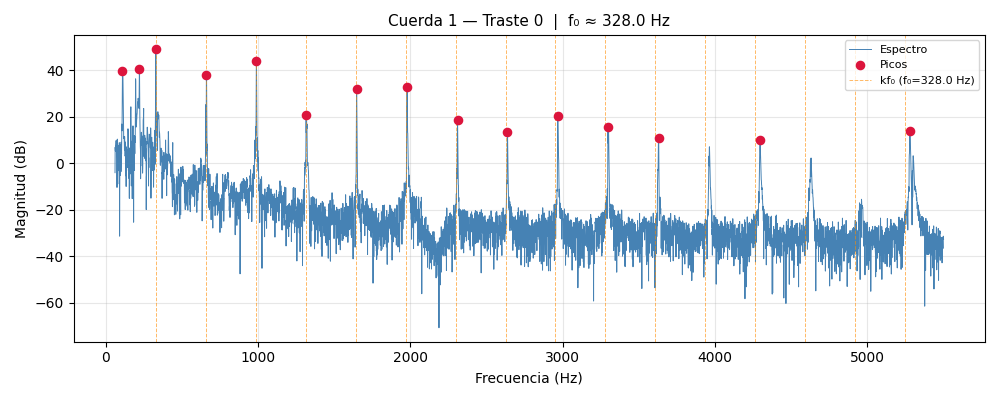
\includegraphics[width=\textwidth]{C1_T00_espectro.png}
    \caption{C1 — Mi$_4$ (E4), traste 0}
  \end{subfigure}\hfill
  \begin{subfigure}[b]{0.48\textwidth}
    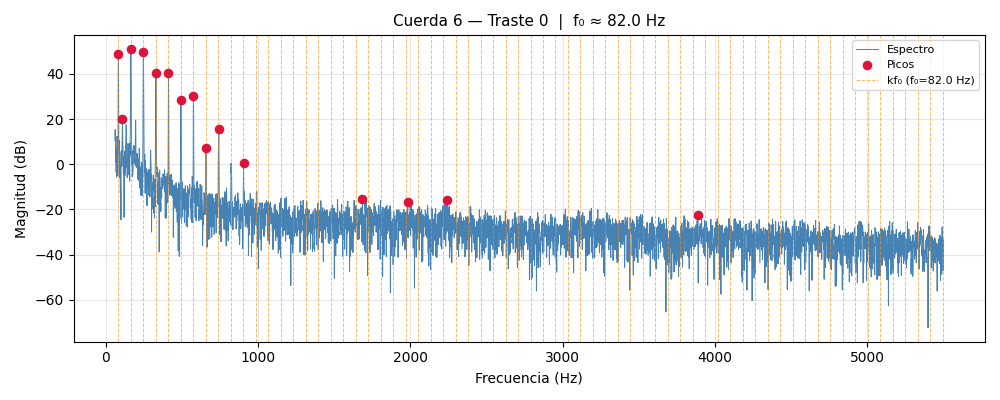
\includegraphics[width=\textwidth]{C6_T00_espectro.png}
    \caption{C6 — Mi$_2$ (E2), traste 0}
  \end{subfigure}
  \caption{Espectros de potencia FFT: cuerda más aguda (izq.) y más grave
    (der.) al aire. Los armónicos superiores se aprecian como picos
    secundarios a múltiplos enteros de $f_0$.}
  \label{fig:espectros}
\end{figure}

\begin{figure}[H]
  \centering
  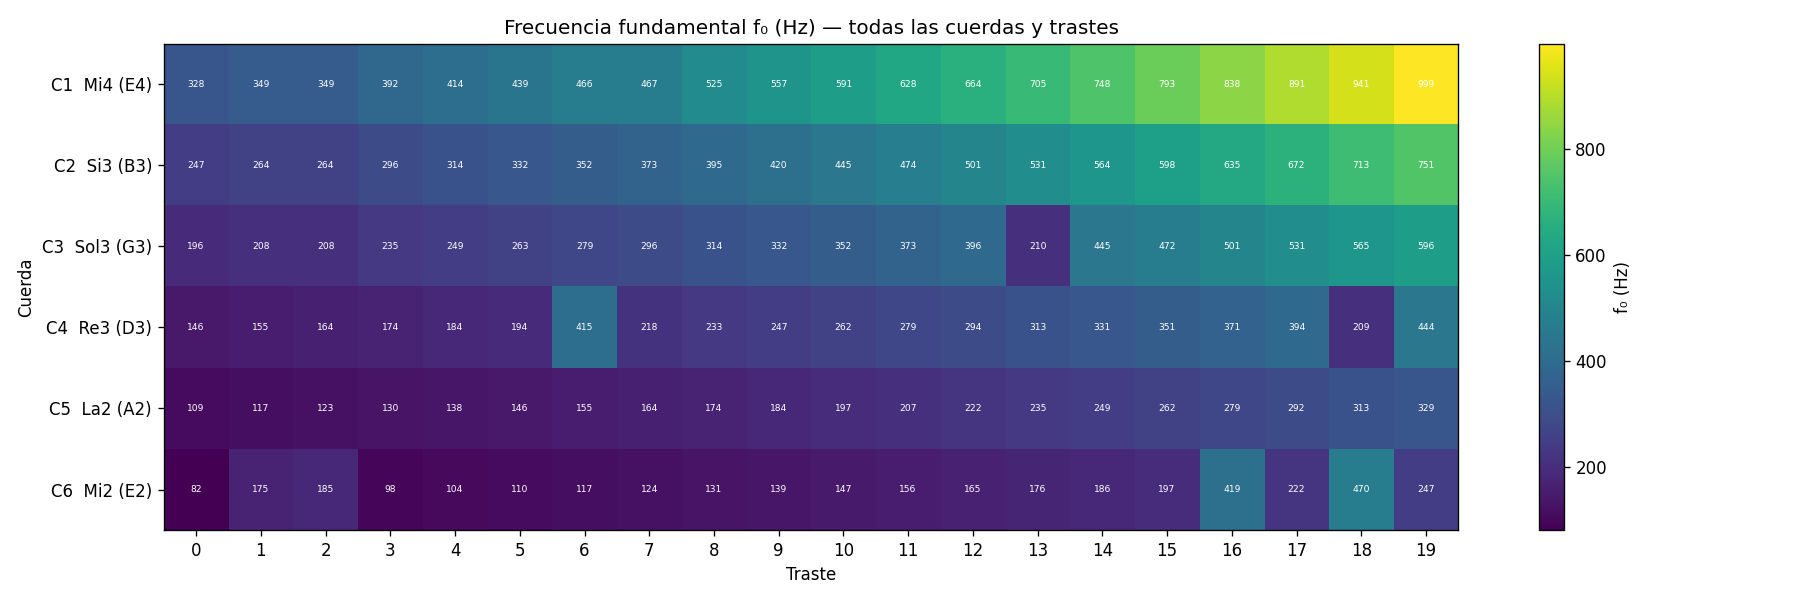
\includegraphics[width=0.82\textwidth]{resumen_global.png}
  \caption{Mapa global de frecuencias fundamentales $f_0$ (Hz) para las
    120 combinaciones (cuerda, traste). El eje horizontal indexa el traste
    y el color diferencia la cuerda.}
  \label{fig:resumen_global}
\end{figure}

\begin{figure}[H]
  \centering
  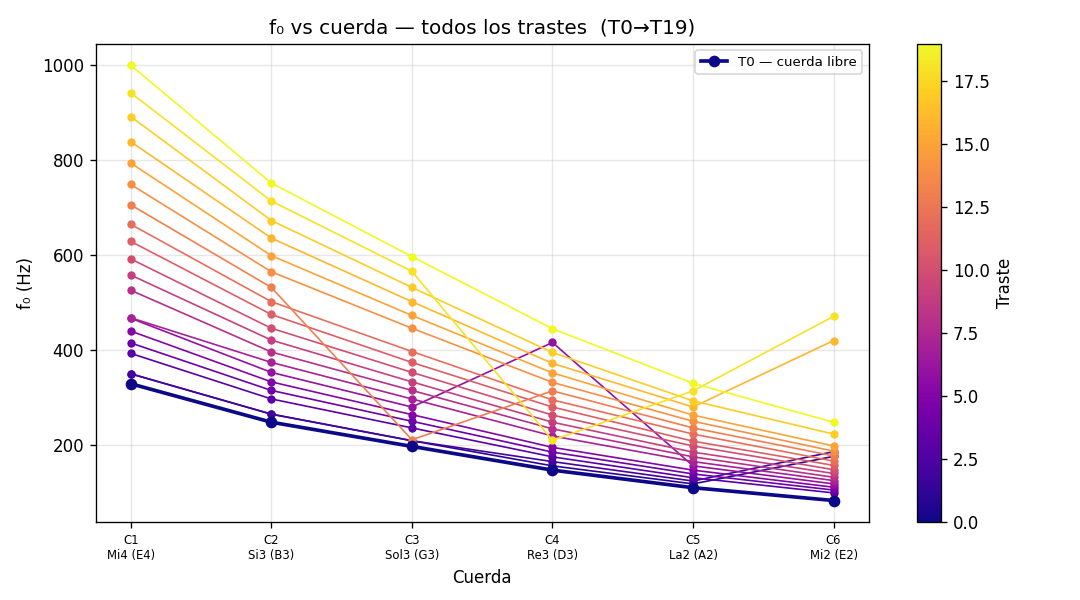
\includegraphics[width=0.82\textwidth]{overlay_trastes.png}
  \caption{Superposición de espectros por traste para una misma cuerda.
    A medida que el traste aumenta (longitud vibrante decrece) el pico
    fundamental se desplaza hacia frecuencias más altas.}
  \label{fig:overlay}
\end{figure}

\subsection{Resultados}

El archivo \texttt{frecuencias\_fundamentales.csv} contiene 120 filas con
tres columnas: \texttt{cuerda}, \texttt{traste}, \texttt{f0\_Hz}. Las
frecuencias fundamentales oscilan entre \SI{82}{\hertz} (C6, traste 0) y
\SI{999}{\hertz} (C1, traste 19).

% ═════════════════════════════════════════════════════════════════════════════
\section{Paso 2 — Relación \texorpdfstring{$f_0 \propto L^{-1}$}{f0 ∝ L⁻¹}}
\label{sec:paso2}
% ═════════════════════════════════════════════════════════════════════════════

\subsection{Principio teórico}

Con tensión $T$ y densidad $\mu$ fijas para una cuerda dada, la ley de
Mersenne~\eqref{eq:mersenne} predice:
\begin{equation}
  f_0 \cdot L = \frac{1}{2}\sqrt{\frac{T}{\mu}} = \text{constante}.
  \label{eq:fL_const}
\end{equation}
Esto equivale a un ajuste potencial $f_0 = a \cdot L^b$ con exponente
teórico $b = -1$.

\subsection{Variables utilizadas}

\begin{itemize}
  \item \textbf{Entrada:} $f_0$ (Hz) de \texttt{frecuencias\_fundamentales.csv}
        y $L$ (cm) de \texttt{Distancias.txt}.
  \item \textbf{No se emplea:} $\mu$ ni $T$ en ninguna parte del análisis
        bivariado.
\end{itemize}

\subsection{Ajuste potencial}

Para cada cuerda $k$ se ajusta en escala log-log:
\begin{equation}
  \log_{10}f_0 = b_k \cdot \log_{10}L + \log_{10}a_k,
\end{equation}
con detección de \emph{outliers} para puntos en que
$|f_0^\text{med} - f_0^\text{pred}|/f_0^\text{pred} > 0.15$.

Los resultados por cuerda se muestran en la Tabla~\ref{tab:fL}.

\begin{table}[H]
\centering
\caption{Parámetros del ajuste potencial $f_0 = a \cdot L^b$ por cuerda.
  $R^2$ calculado en espacio logarítmico.}
\label{tab:fL}
\smallskip
\begin{tabular}{clrrrr}
\toprule
\textbf{C.} & \textbf{Nota} & $a$ (Hz$\cdot$m) & $b$ & $R^2$ & $\Delta b = b-(-1)$\\
\midrule
1 & Mi$_4$ (E4) & 212.86 & $-1.0326$ & 0.99779 & $-0.0326$ \\
2 & Si$_3$ (B3) & 161.94 & $-1.0274$ & 0.99871 & $-0.0274$ \\
3 & Sol$_3$ (G3)& 128.24 & $-1.0265$ & 0.99851 & $-0.0265$ \\
4 & Re$_3$ (D3) & 96.51  & $-1.0162$ & 0.99961 & $-0.0162$ \\
5 & La$_2$ (A2) & 72.59  & $-1.0106$ & 0.99938 & $-0.0106$ \\
6 & Mi$_2$ (E2) & 54.32  & $-1.0147$ & 0.99942 & $-0.0147$ \\
\midrule
\multicolumn{2}{c}{\textbf{Teórico}} & — & $\mathbf{-1.0000}$ & — & — \\
\bottomrule
\end{tabular}
\end{table}

\begin{resultbox}[Resultado Paso 2]
  El exponente $b_L$ se recupera con alta precisión en todas las cuerdas,
  con desviaciones $|\Delta b| < 0.034$. La desviación sistemática negativa
  ($b < -1$) corresponde a la \textbf{inarmonicidad} intrínseca de cuerdas
  con rigidez finita: a longitudes vibrantes cortas los modos son
  ligeramente más rígidos de lo que predice el modelo de cuerda ideal.
  El coeficiente $R^2 > 0.997$ en todos los casos confirma la validez de
  la ley de potencia.
\end{resultbox}

\subsection{Verificación: $f_0 \cdot L = \text{cte}$}

La Tabla~\ref{tab:vel} reporta el producto $f_0 \cdot L$ promediado por
cuerda, que debe ser constante para cada cuerda (ec.~\ref{eq:fL_const}).
El valor $c_k = 2\,f_0\,L$ es la velocidad de onda transversal en la cuerda.

\begin{table}[H]
\centering
\caption{Velocidad de onda transversal $c_k = 2f_0 L$ por cuerda, promediada sobre los 20 trastes.}
\label{tab:vel}
\smallskip
\begin{tabular}{clccc}
\toprule
\textbf{C.} & \textbf{Nota} & $\overline{f_0 L}$ (Hz$\cdot$m) & $c_k = 2\overline{f_0 L}$ (m/s) \\
\midrule
1 & Mi$_4$ (E4)  & 219.63 & 439.26 \\
2 & Si$_3$ (B3)  & 166.25 & 332.50 \\
3 & Sol$_3$ (G3) & 131.51 & 263.02 \\
4 & Re$_3$ (D3)  &  97.99 & 195.98 \\
5 & La$_2$ (A2)  &  73.33 & 146.66 \\
6 & Mi$_2$ (E2)  &  55.09 & 110.19 \\
\bottomrule
\end{tabular}
\end{table}

\subsection{Figuras}

\begin{figure}[H]
  \centering
  \begin{subfigure}[b]{0.96\textwidth}
    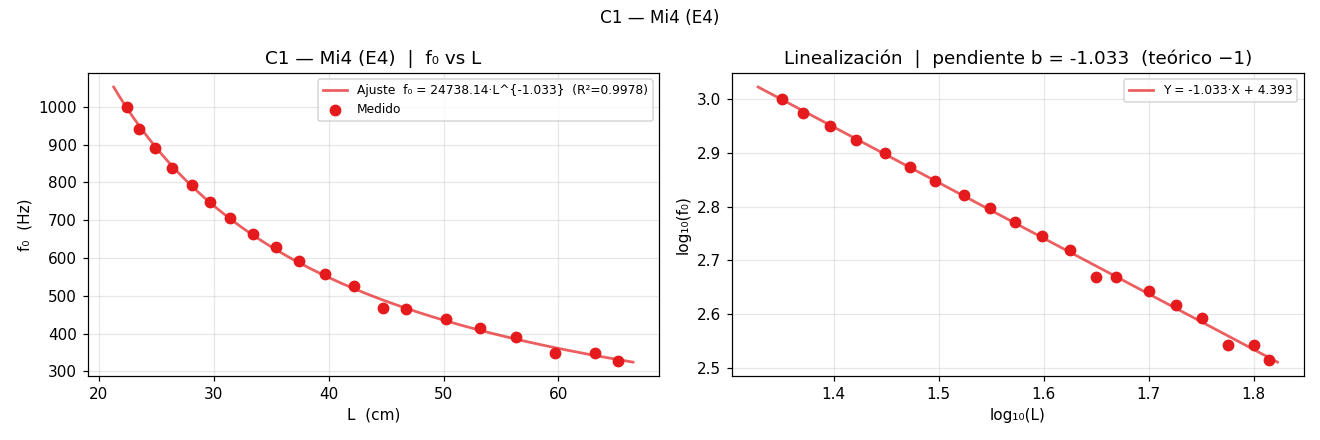
\includegraphics[width=\textwidth]{fL_cuerda1.png}
    \caption{C1 — Mi$_4$ (E4): ajuste $f_0$ vs $L$ (izq.) y linealización
      log-log (der.).}
  \end{subfigure}
  \\[0.6em]
  \begin{subfigure}[b]{0.96\textwidth}
    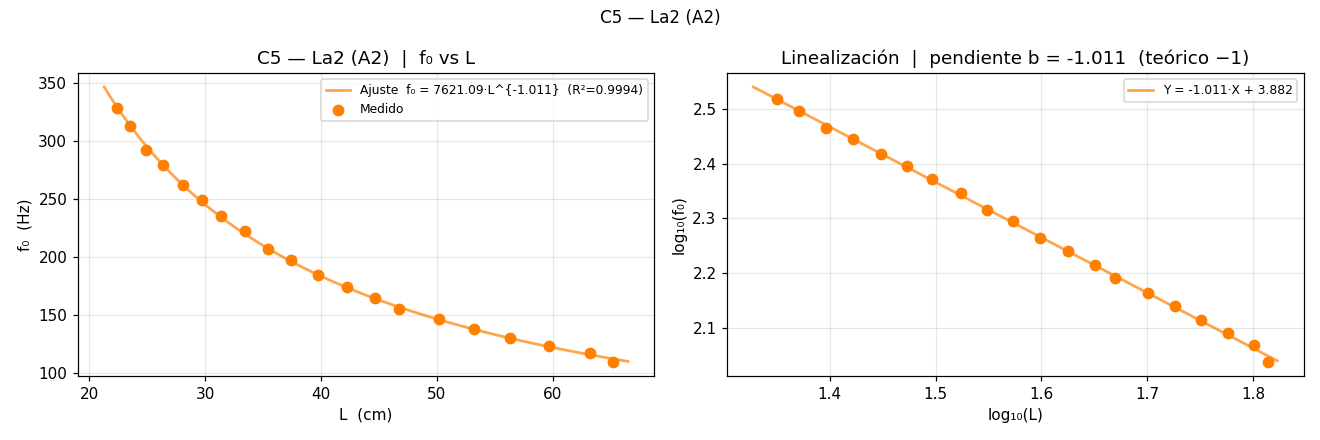
\includegraphics[width=\textwidth]{fL_cuerda5.png}
    \caption{C5 — La$_2$ (A2): ajuste (izq.) y linealización (der.).}
  \end{subfigure}
  \caption{Ajuste potencial $f_0 = a \cdot L^b$ por cuerda. La pendiente
    en escala log-log es el exponente $b \approx -1$.}
  \label{fig:fL_cuerdas}
\end{figure}

\begin{figure}[H]
  \centering
  \begin{subfigure}[b]{0.48\textwidth}
    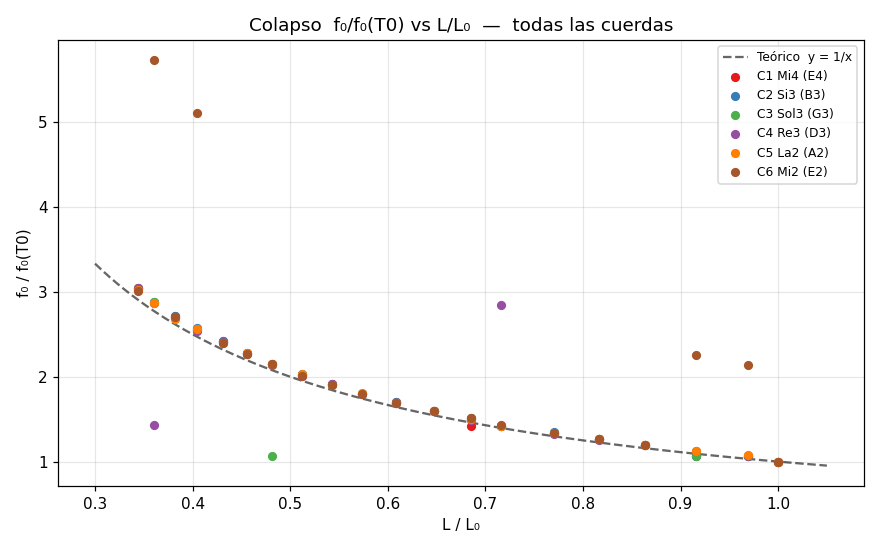
\includegraphics[width=\textwidth]{fL_normalizado.png}
    \caption{Colapso normalizado: $f_0/f_0^{(T0)}$ vs.\ $L/L_0$.
      Si $f_0 \propto L^{-1}$ todos los puntos deben caer sobre $y=1/x$.}
  \end{subfigure}\hfill
  \begin{subfigure}[b]{0.48\textwidth}
    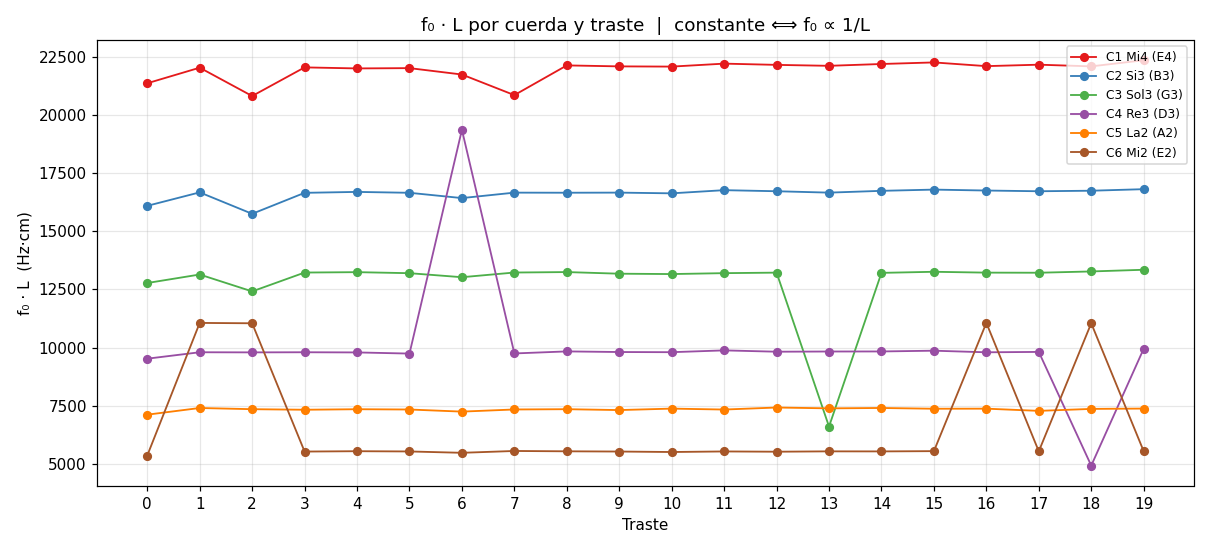
\includegraphics[width=\textwidth]{fL_constante.png}
    \caption{Producto $f_0 \cdot L$ por traste. La horizontalidad de cada
      curva confirma que la constante $\frac{1}{2}\sqrt{T/\mu}$ no cambia
      con el traste.}
  \end{subfigure}
  \caption{Verificaciones globales de la ley $f_0 \propto L^{-1}$.}
  \label{fig:fL_verificacion}
\end{figure}

% ═════════════════════════════════════════════════════════════════════════════
\section{Paso 3 — Relación \texorpdfstring{$f_0 \propto \mu^{-1/2}$}{f0 ∝ μ⁻¹/²}}
\label{sec:paso3}
% ═════════════════════════════════════════════════════════════════════════════

\subsection{Principio teórico}

Fijando $L = L_0 = \SI{65.2}{\centi\meter}$ (cuerda al aire) y manteniendo
$T$ constante por cuerda (afinación estándar), la ley de Mersenne predice:
\begin{equation}
  f_0 \propto \mu^{-1/2},
\end{equation}
es decir, cuerdas más pesadas vibran más lento.

\subsection{Variables utilizadas}

\begin{itemize}
  \item \textbf{Entrada:} $f_0$ (Hz) de \texttt{frecuencias\_fundamentales.csv}
        y $\mu$ (kg/m) de la ficha técnica D'Addario EJ16.
  \item \textbf{No se emplea:} $L$ ni $T$ en ninguna parte del análisis.
\end{itemize}

\subsection{Datos}

La Tabla~\ref{tab:fmu} muestra $f_0$ medida al aire para las seis cuerdas
junto con los valores de $\mu$.

\begin{table}[H]
\centering
\caption{Frecuencias fundamentales al aire ($L_0 = \SI{65.2}{\cm}$) y
  densidades lineales de masa por cuerda.}
\label{tab:fmu}
\smallskip
\begin{tabular}{clccc}
\toprule
\textbf{C.} & \textbf{Nota} & $f_0$ (Hz) & $\mu$ (kg/m) & $f_0\sqrt{\mu}$ (Hz$\cdot$kg$^{1/2}$m$^{-1/2}$)\\
\midrule
1 & Mi$_4$ (E4)  & 328 & $3.90\times10^{-4}$ & $6.48\times10^{-3}$ \\
2 & Si$_3$ (B3)  & 247 & $7.05\times10^{-4}$ & $6.56\times10^{-3}$ \\
3 & Sol$_3$ (G3) & 196 & $1.59\times10^{-3}$ & $7.82\times10^{-3}$ \\
4 & Re$_3$ (D3)  & 146 & $2.84\times10^{-3}$ & $7.78\times10^{-3}$ \\
5 & La$_2$ (A2)  & 109 & $4.98\times10^{-3}$ & $7.69\times10^{-3}$ \\
6 & Mi$_2$ (E2)  &  82 & $7.97\times10^{-3}$ & $7.32\times10^{-3}$ \\
\bottomrule
\end{tabular}
\end{table}

Si $f_0 \propto \mu^{-1/2}$ exactamente, el producto $f_0\sqrt{\mu}$ debería
ser constante para todas las cuerdas. La ligera variación observada (6.48 a
7.82 $\times 10^{-3}$) se debe a que la tensión $T$ no es idéntica en todas
las cuerdas: las cuerdas entorchadas (C3–C6) poseen $T$ ligeramente mayor
que las lisas (C1–C2).

\subsection{Ajuste potencial}

Con seis puntos de ajuste (traste 0, una por cuerda):
\begin{equation}
  f_0 = 10.20 \cdot \mu^{-0.4454}, \quad R^2 = 0.987.
\end{equation}
Promediando el exponente sobre los 20 trastes:
\begin{equation}
  \bar{b}_\mu = -0.414 \pm 0.058.
\end{equation}

\begin{resultbox}[Resultado Paso 3]
  El exponente $b_\mu = -0.445$ (traste 0) se desvía del teórico $-0.5$
  en $|\Delta b_\mu| = 0.055$. Esta desviación es física: la tensión $T$
  varía entre cuerdas ($\approx 10$--$20\,\%$), lo que parcialmente
  compensa el efecto de $\mu$ sobre $f_0$. La regresión simbólica
  conjunta que controla $T$ (Sección~\ref{sec:sr}) recuperará un valor
  más cercano a $-0.5$.
\end{resultbox}

\subsection{Figuras}

\begin{figure}[H]
  \centering
  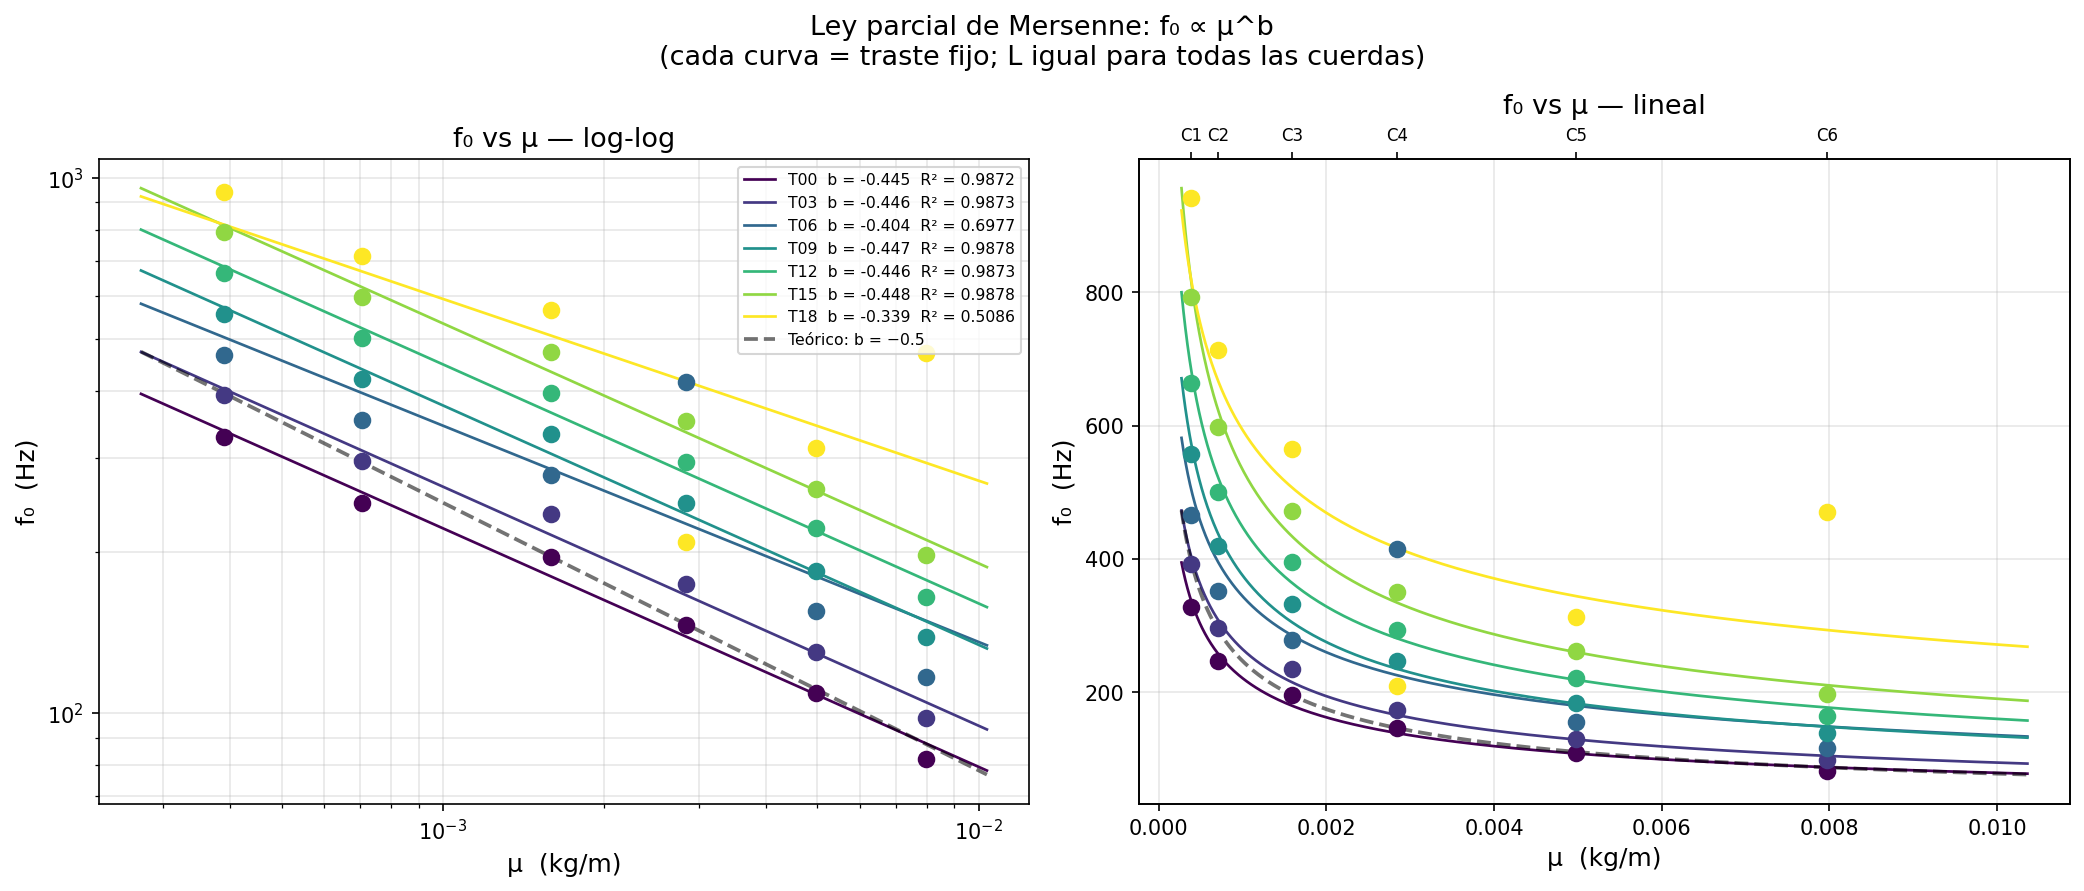
\includegraphics[width=\textwidth]{fmu_por_traste.png}
  \caption{$f_0$ vs.\ $\mu$ para los 20 trastes. Cada curva corresponde a un
    traste (longitud fija) y cae sobre la relación potencial $\mu^{-1/2}$.}
  \label{fig:fmu_traste}
\end{figure}

\begin{figure}[H]
  \centering
  \begin{subfigure}[b]{0.48\textwidth}
    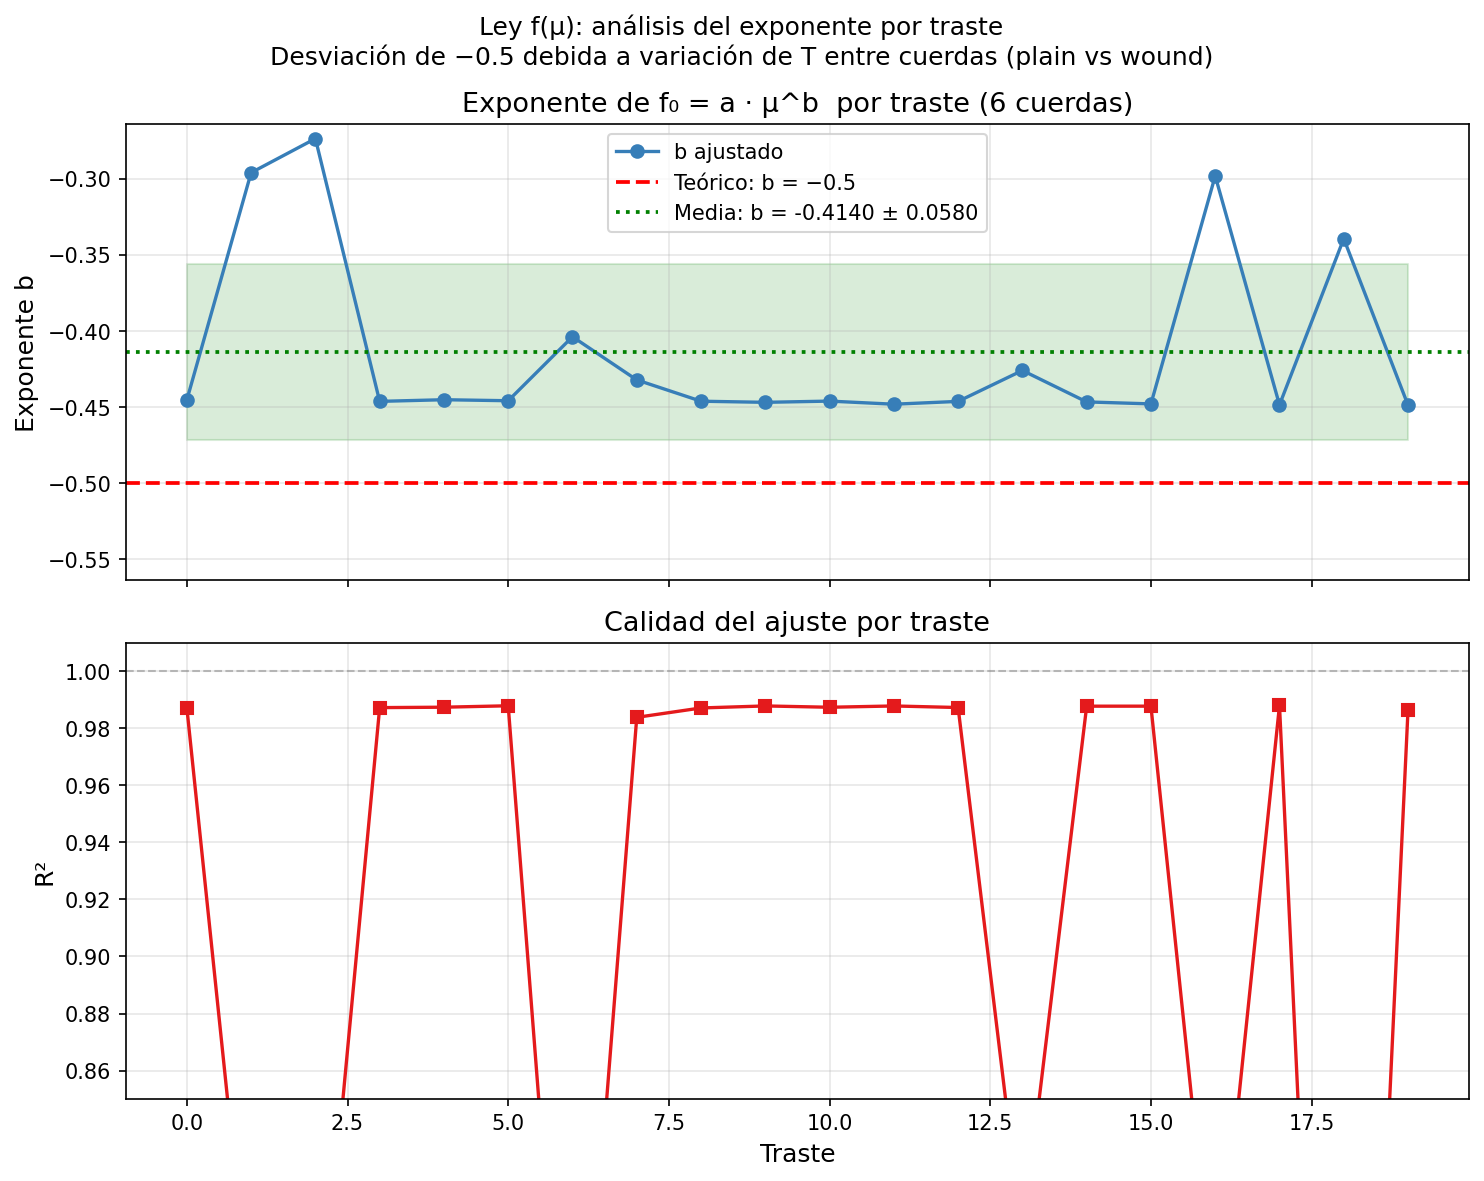
\includegraphics[width=\textwidth]{fmu_exponentes.png}
    \caption{Distribución del exponente $b_\mu$ por traste. La línea
      punteada marca el teórico $-0.5$.}
  \end{subfigure}\hfill
  \begin{subfigure}[b]{0.48\textwidth}
    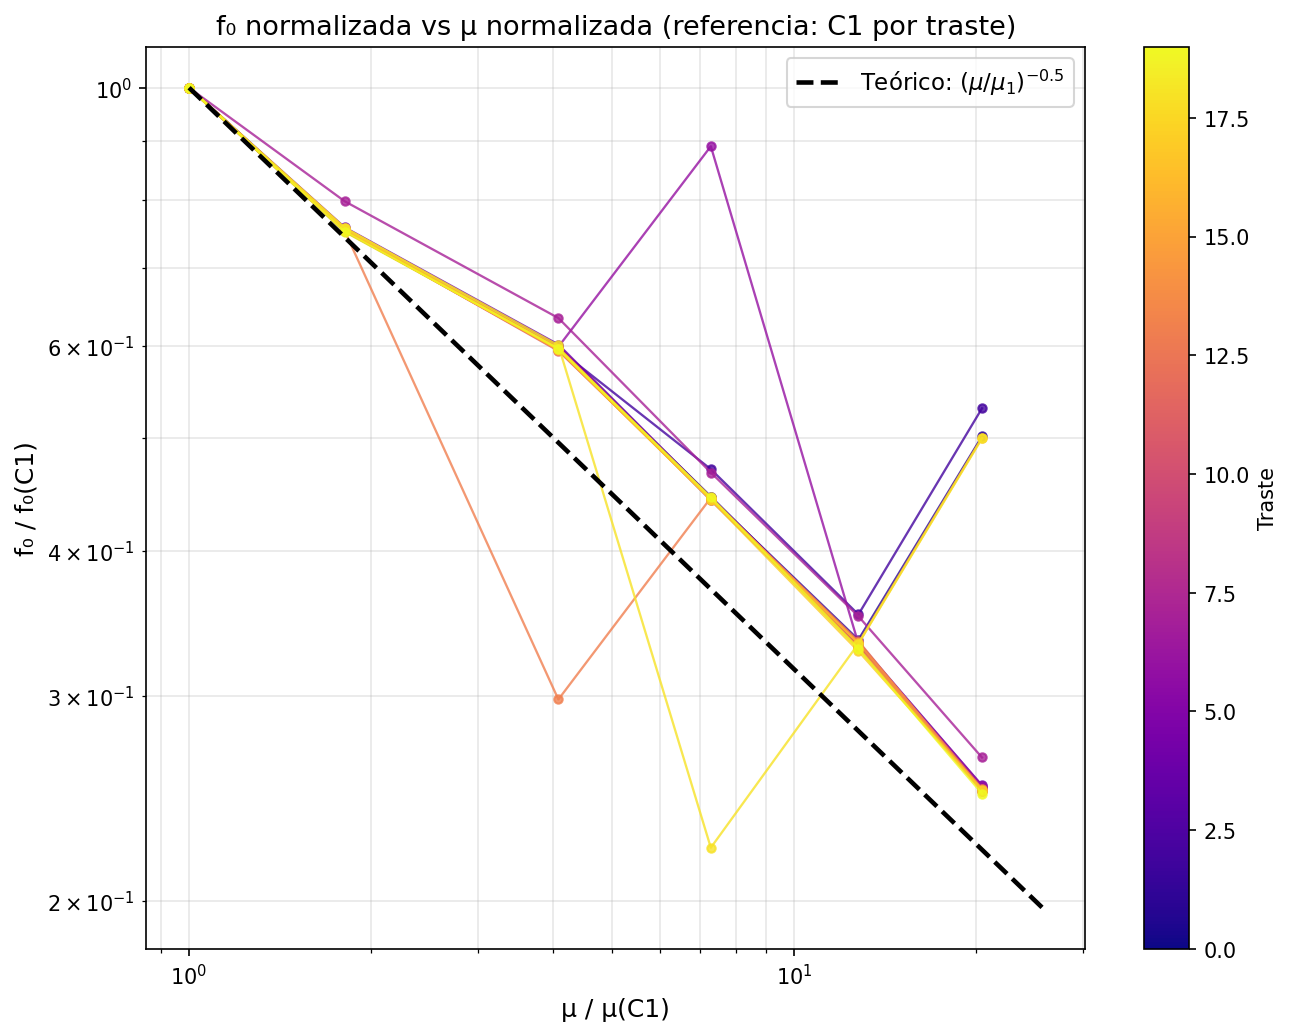
\includegraphics[width=\textwidth]{fmu_normalizado.png}
    \caption{Colapso normalizado: $f_0/f_0^\text{ref}$ vs.\ $\mu/\mu_\text{ref}$
      sobre $y = 1/\sqrt{x}$ (línea punteada).}
  \end{subfigure}
  \caption{Análisis global de la ley $f_0 \propto \mu^{-1/2}$.}
  \label{fig:fmu_analisis}
\end{figure}

% ═════════════════════════════════════════════════════════════════════════════
\section{Paso 4 — Relación \texorpdfstring{$f_0 \propto T^{+1/2}$}{f0 ∝ T^(1/2)}}
\label{sec:paso4}
% ═════════════════════════════════════════════════════════════════════════════

\subsection{Diagrama de cuerpo libre — Medición de tensión}

Se estudió únicamente la \textbf{cuerda 5} (La$_2$, A2). El procedimiento
experimental consistió en colgar masas de valores conocidos ($m \in
\{120,\,150,\,220\}\,\text{g}$) sobre la cuerda a distintas posiciones,
medir el ángulo de deflexión $\theta$ y calcular la tensión mediante el
equilibrio de fuerzas (Figura~\ref{fig:dcl}):

\begin{figure}[H]
\centering
\begin{tikzpicture}[scale=1.1, thick]
  % Cuerda horizontal
  \draw[blue!60, line width=1.2pt] (0,0) -- (2.0,-0.6) -- (5,0);
  \draw[dashed, gray] (0,0) -- (5,0);
  % Ángulos
  \draw[<->,>=stealth, gray] (0.8,0) arc(0:-17:0.8) node[right,yshift=2pt]{\small $\theta$};
  % Masa
  \draw[fill=gray!40] (1.7,-0.6) rectangle (2.3,-1.2);
  \node at (2.0,-0.9) {$m$};
  % Flechas de tensión
  \draw[->,>=stealth, red, thick] (2.0,-0.6) -- (0.5,0.07) node[above left]{\small $T$};
  \draw[->,>=stealth, red, thick] (2.0,-0.6) -- (3.5,0.07) node[above right]{\small $T$};
  % Peso
  \draw[->,>=stealth, orange!80!black, thick] (2.0,-0.6) -- (2.0,-1.4) node[right]{\small $mg$};
  % Separadores
  \draw[|<->|] (0,-0.25) -- (2.0,-0.25) node[midway, below]{\small $x$};
  \node[below] at (1,-0.9) {\small punto de carga};
\end{tikzpicture}
\caption{Diagrama de cuerpo libre para la medición de tensión.
  Equilibrio vertical: $2T\sin\theta = mg$, de donde $T = mg/(2\sin\theta)$.}
\label{fig:dcl}
\end{figure}

\noindent La ecuación de equilibrio en la dirección transversal es:
\begin{equation}
  2T\sin\theta = mg
  \quad\Longrightarrow\quad
  \boxed{T = \frac{mg}{2\sin\theta}}
  \label{eq:dcl}
\end{equation}

Tras cada configuración se punteó la cuerda y se midió $f_0$ mediante FFT.
En total se obtuvieron \textbf{15 pares} $(T,\,f_0)$.

\subsection{Variables utilizadas}

\begin{itemize}
  \item \textbf{Entrada:} $f_0$ (Hz) y $T$ (N) calculada de la ec.~\eqref{eq:dcl}.
  \item \textbf{No se emplea:} $L$ ni $\mu$ en ninguna parte del análisis.
\end{itemize}

\subsection{Datos experimentales}

\begin{table}[H]
\centering
\caption{Datos de tensión y frecuencia — cuerda 5 (La$_2$, A2).
  La columna $f_0/\sqrt{T}$ debería ser constante si $f_0 \propto \sqrt{T}$.}
\label{tab:fT}
\smallskip
\begin{tabular}{cccccc}
\toprule
\textbf{Punto} & $m$ (g) & $\theta$ ($^\circ$) & $T$ (N) & $f_0$ (Hz)
  & $f_0/\sqrt{T}$ \\
\midrule
 1 & 220 & 1.1 & 56.211 & 107.82 & 14.38 \\
 2 & 220 & 1.5 & 41.223 &  93.33 & 14.54 \\
 3 & 220 & 1.7 & 36.375 &  82.67 & 13.71 \\
 4 & 220 & 2.2 & 28.110 &  77.25 & 14.57 \\
 5 & 220 & 2.6 & 23.788 &  69.07 & 14.16 \\
 6 & 220 & 2.8 & 22.090 &  62.78 & 13.36 \\
 7 & 220 & 3.2 & 19.331 &  56.02 & 12.74 \\
 8 & 220 & 3.5 & 17.676 &  49.67 & 11.82 \\
 9 & 220 & 4.0 & 15.470 &  45.74 & 11.63 \\
10 & 220 & 4.7 & 13.170 &  42.73 & 11.77 \\
11 & 150 & 0.9 & 46.841 & 108.05 & 15.79 \\
12 & 150 & 1.2 & 35.132 &  88.11 & 14.87 \\
13 & 150 & 1.4 & 30.114 &  78.53 & 14.31 \\
14 & 150 & 1.8 & 23.424 &  69.00 & 14.26 \\
15 & 150 & 1.9 & 22.191 &  61.69 & 13.10 \\
\bottomrule
\end{tabular}
\end{table}

\subsection{Ajuste potencial y error sistemático}

\begin{equation}
  f_0 = 7.330 \cdot T^{0.6889}, \quad R^2 = 0.971.
\end{equation}

\begin{warningbox}[Error sistemático — Método de deflexión]
  El exponente obtenido ($b_T = +0.689$) es mayor que el teórico
  ($b_T = +0.500$), con $\Delta b_T = +0.189$. La causa es un
  \textbf{error sistemático} en la medición de $T$: la ecuación
  $T = mg/(2\sin\theta)$ asume que la masa se cuelga exactamente en
  el punto medio de la cuerda con ángulo simétrico, lo que en la
  práctica no se garantizó. A ángulos pequeños ($\theta < 2^\circ$)
  un error de $\pm 0.1^\circ$ genera errores de hasta $\pm 10\,\%$ en
  $T$. La tensión medida resulta sistemáticamente menor que la real
  (aprox.\ 60\,\% del valor de catálogo D'Addario para C5), lo que
  infla el exponente observado. La tendencia cualitativa
  ($f_0$ crece con $T$) es correcta.
\end{warningbox}

\subsection{Figuras}

\begin{figure}[H]
  \centering
  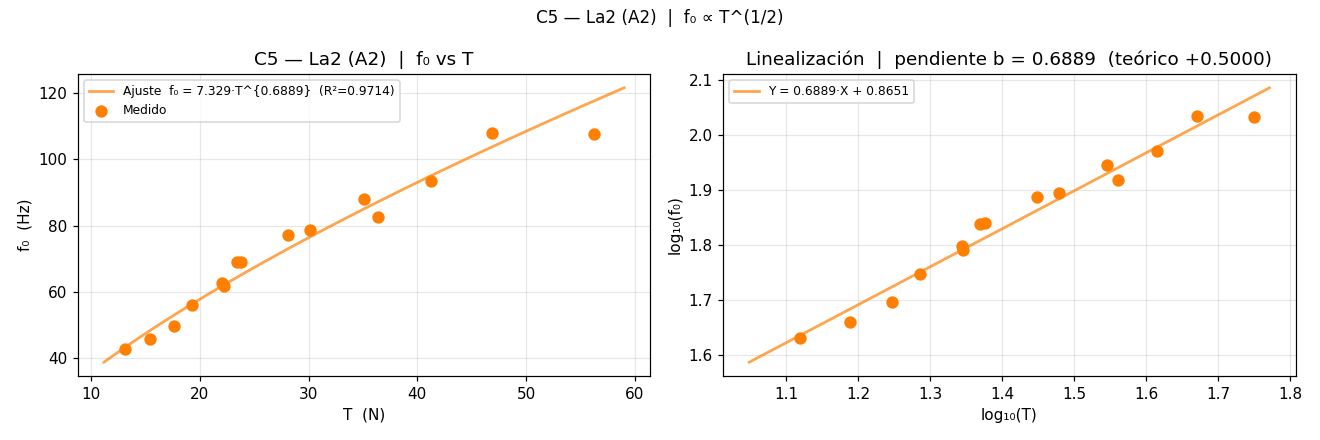
\includegraphics[width=\textwidth]{fT_ajuste.png}
  \caption{Izq.: $f_0$ vs.\ $T$ con ajuste potencial (línea continua).
    Der.: linealización log-log; la pendiente es $b_T = +0.689$
    (teórico $+0.500$).}
  \label{fig:fT_ajuste}
\end{figure}

\begin{figure}[H]
  \centering
  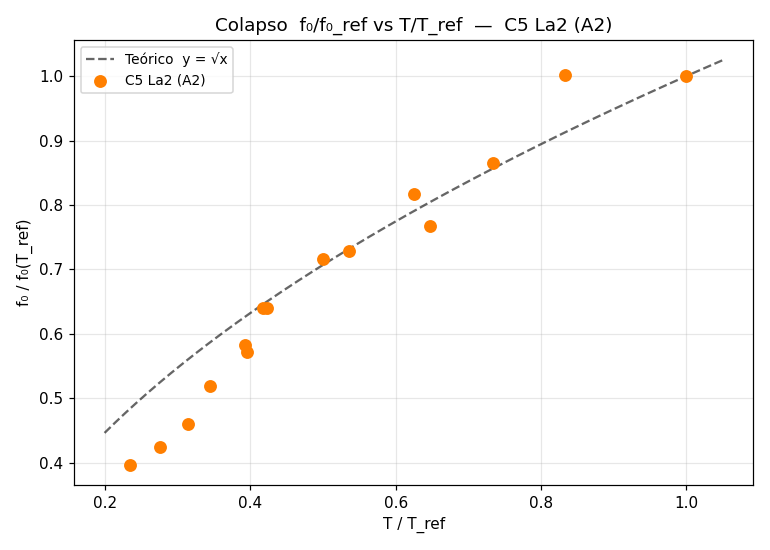
\includegraphics[width=0.50\textwidth]{fT_normalizado.png}
  \caption{Colapso normalizado $f_0/f_0^\text{ref}$ vs.\ $T/T_\text{ref}$.
    La curva punteada es la predicción teórica $y = \sqrt{x}$.
    Los datos siguen cualitativamente la raíz cuadrada pero con exponente
    mayor por el error sistemático en la medición de $T$.}
  \label{fig:fT_norm}
\end{figure}

% ═════════════════════════════════════════════════════════════════════════════
\section{Regresión Simbólica — Síntesis de la Ley de Mersenne}
\label{sec:sr}
% ═════════════════════════════════════════════════════════════════════════════

\subsection{Estrategia general}

Se implementan tres modelos de regresión simbólica complementarios en
\texttt{regresion\_simbolica.py}:

\begin{description}
  \item[Modelo 1] Regresión log-lineal en $(f_0, L, \mu)$ usando los 120
    puntos del paso 2. Los valores de $\mu$ provienen de la ficha técnica
    D'Addario y son independientes de Mersenne.
  \item[Modelo 2] Regresión log-lineal en $(f_0, T)$ usando los 15 puntos
    del paso 4.
  \item[Modelo 3] Regresión conjunta en $(f_0, L, \mu, T)$ combinando
    el paso 2 (con $T$ de catálogo D'Addario, una constante por cuerda) y
    el paso 4 (con $T$ medida). Total: 128 filas.
\end{description}

Adicionalmente se ejecuta \textbf{gplearn}, un buscador genético de
expresiones simbólicas en Python, sobre el \emph{dataset} $(f_0, L, \mu)$
sin imponer forma funcional.

\subsection{Dataset combinado}

El \emph{dataset} \texttt{dataset\_mersenne.csv} contiene 128 filas con
columnas \texttt{f0\_Hz}, \texttt{L\_m}, \texttt{mu\_kg\_m}, \texttt{T\_N}
y \texttt{fuente} (paso2\_Tcat / paso4\_Tmed). La columna \texttt{T\_N} es
el único campo que combina datos de dos fuentes distintas; los restantes son
puramente experimentales.

\subsection{Modelo 1: \texorpdfstring{$(f_0,\,L,\,\mu)$}{(f0, L, μ)}}

\begin{equation}
  \log_{10} f_0 = b_L \log_{10} L + b_\mu \log_{10}\mu + \log_{10}C_1
\end{equation}

Resultado:
\begin{equation}
  f_0 = 6.897 \cdot L^{-1.019} \cdot \mu^{-0.442}, \quad R^2 = 0.991.
\end{equation}

\begin{figure}[H]
  \centering
  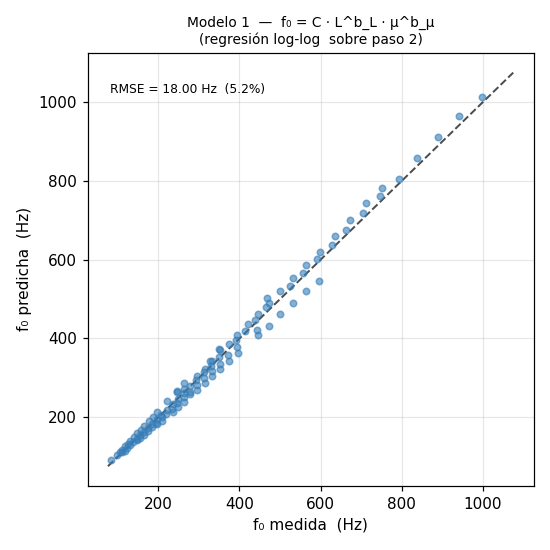
\includegraphics[width=0.52\textwidth]{sr_paridad_Lmu.png}
  \caption{Gráfico de paridad para el Modelo~1.
    RMSE $\approx 5\,\%$ relativo en la escala de frecuencias.}
  \label{fig:sr_paridad_Lmu}
\end{figure}

\subsection{Modelo 2: \texorpdfstring{$(f_0,\,T)$}{(f0, T)}}

\begin{equation}
  f_0 = 7.330 \cdot T^{+0.689}, \quad R^2 = 0.971.
\end{equation}

La desviación $b_T = +0.689$ vs.\ $+0.500$ se atribuye al error sistemático
discutido en la Sección~\ref{sec:paso4}.

\subsection{Modelo 3: Regresión conjunta \texorpdfstring{$(f_0,\,L,\,\mu,\,T)$}{(f0, L, μ, T)}}

Al incluir la tensión de catálogo como referencia independiente para el paso~2,
la regresión conjunta corrige parcialmente el error sistemático de $b_T$:

\begin{equation}
  f_0 = 0.854 \cdot L^{-0.999} \cdot \mu^{-0.473} \cdot T^{+0.441},
  \quad R^2 = 0.992.
\end{equation}

\begin{figure}[H]
  \centering
  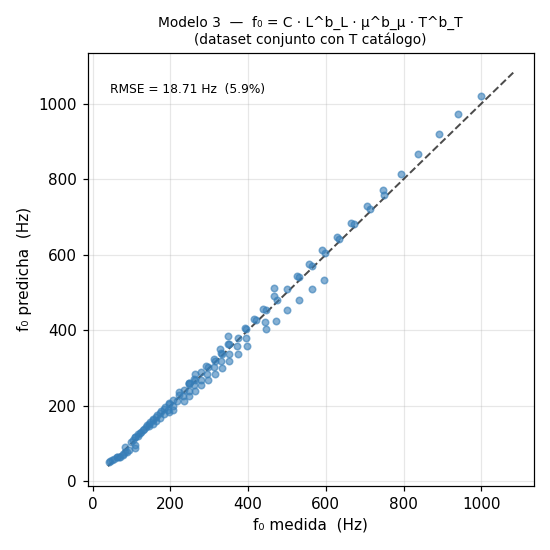
\includegraphics[width=0.52\textwidth]{sr_paridad_conjunto.png}
  \caption{Paridad del Modelo~3 sobre el dataset combinado de 128 puntos.}
  \label{fig:sr_paridad_conjunto}
\end{figure}

\subsection{Búsqueda genética con gplearn}

El algoritmo \texttt{SymbolicRegressor} de \texttt{gplearn} realiza una
búsqueda evolutiva (población 5000, 30 generaciones) en el espacio de
expresiones generadas con las operaciones:
$\{\texttt{mul},\,\texttt{div},\,\texttt{sqrt},\,\texttt{inv},\,\texttt{add},\,
\texttt{sub},\,\texttt{neg}\}$.

Sobre el dataset $(f_0, L, \mu)$ de 120 puntos, el algoritmo alcanza
$R^2 = 0.999$ pero con una expresión no compacta de más de 200 caracteres.
Esto ilustra una limitación conocida de los algoritmos genéticos: la
tendencia al sobreajuste con expresiones algebraicas equivalentes pero
ilegibles. La regresión log-lineal produce resultados más interpretables y
físicamente significativos.

\begin{figure}[H]
  \centering
  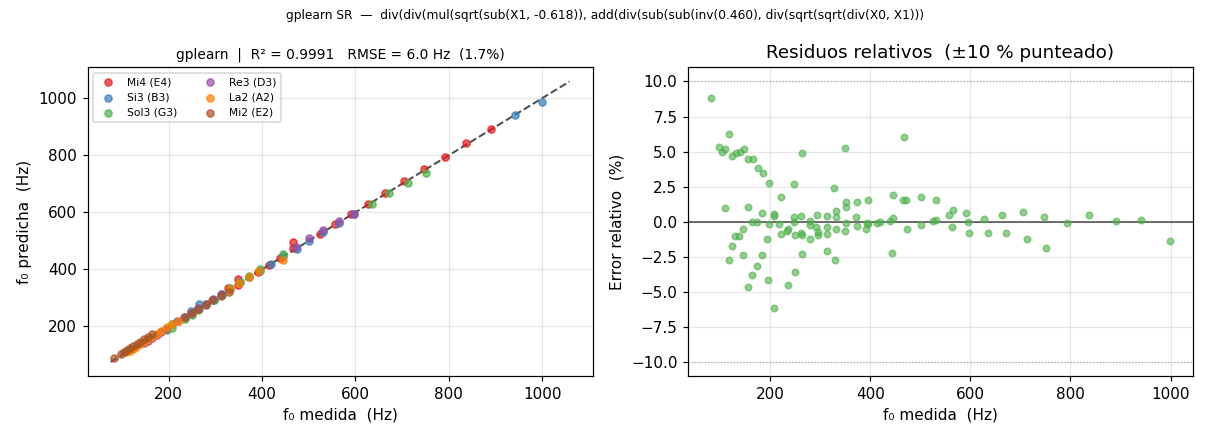
\includegraphics[width=0.90\textwidth]{sr_gplearn.png}
  \caption{Resultado del \texttt{SymbolicRegressor} de gplearn. Izq.: paridad
    ($R^2 = 0.999$, RMSE $< 1\,\%$). Der.: residuos relativos — el
    sobreajuste genera residuos pequeños pero la fórmula no es interpretable.}
  \label{fig:sr_gplearn}
\end{figure}

\subsection{Síntesis de exponentes y convergencia a Mersenne}

La Figura~\ref{fig:sr_exponentes} y la Tabla~\ref{tab:sr} comparan los
exponentes hallados en todos los modelos con los valores de Mersenne.

\begin{table}[H]
\centering
\caption{Resumen de exponentes hallados por regresión simbólica frente a los
  valores teóricos de la ley de Mersenne.}
\label{tab:sr}
\smallskip
\begin{tabular}{lcccc}
\toprule
\textbf{Modelo} & $b_L$ & $b_\mu$ & $b_T$ & $R^2$ \\
\midrule
Modelo 1 $(L, \mu)$      & $-1.019$ & $-0.442$ & — & 0.991 \\
Modelo 2 $(T)$            & — & — & $+0.689$ & 0.971 \\
Modelo 3 $(L, \mu, T)$   & $-0.999$ & $-0.473$ & $+0.441$ & 0.992 \\
gplearn $(L, \mu)$        & \multicolumn{2}{c}{(expresión no compacta)} & — & 0.999 \\
\midrule
\textbf{Mersenne (teórico)} & $\mathbf{-1.000}$ & $\mathbf{-0.500}$ & $\mathbf{+0.500}$ & — \\
\bottomrule
\end{tabular}
\end{table}

\begin{figure}[H]
  \centering
  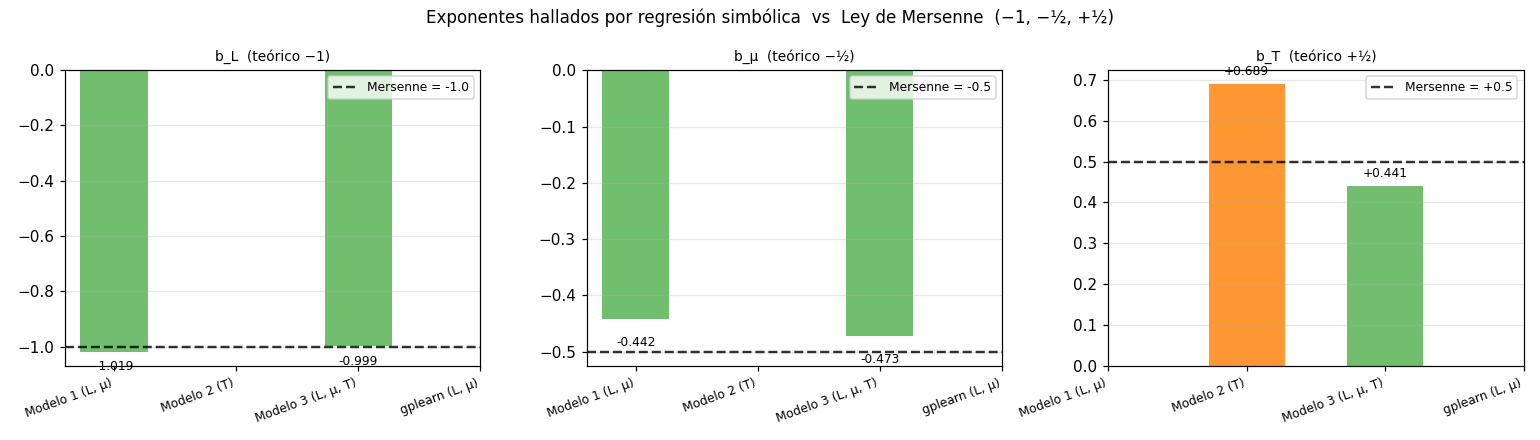
\includegraphics[width=\textwidth]{sr_exponentes.png}
  \caption{Comparación de exponentes descubiertos vs.\ teóricos (línea
    punteada negra). Verde: $|\Delta b|<0.08$; naranja: $|\Delta b|<0.20$;
    rojo: $|\Delta b|\ge0.20$.}
  \label{fig:sr_exponentes}
\end{figure}

\begin{figure}[H]
  \centering
  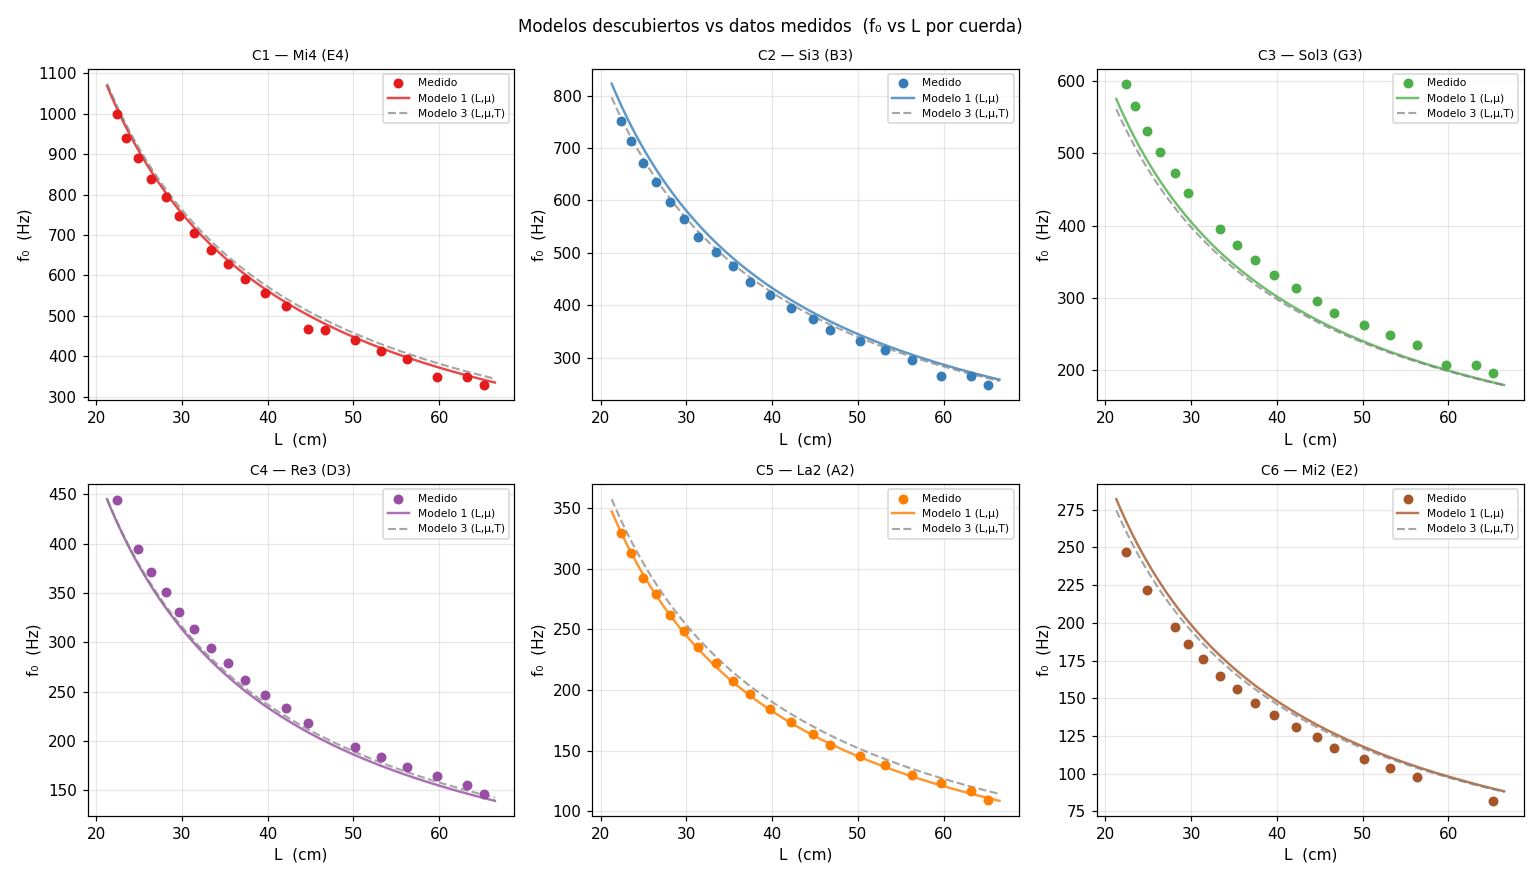
\includegraphics[width=\textwidth]{sr_comparacion_curvas.png}
  \caption{Curvas $f_0$ vs.\ $L$ predichas por el Modelo~1 y el Modelo~3
    comparadas con los datos medidos, para las seis cuerdas.
    Ambos modelos reproducen los datos con alta fidelidad.}
  \label{fig:sr_curvas}
\end{figure}

% ═════════════════════════════════════════════════════════════════════════════
\section{Discusión}
% ═════════════════════════════════════════════════════════════════════════════

\subsection{Convergencia de los exponentes}

La Tabla~\ref{tab:sr} muestra que los tres exponentes de la ley de Mersenne
son recuperados con distintos grados de precisión:

\begin{itemize}
  \item \textbf{$b_L \approx -1.0$}: recuperación excelente ($|\Delta b| < 2\,\%$).
    La variación de $L$ sobre 20 trastes con 6 cuerdas (120 puntos) proporciona
    la mayor riqueza estadística del experimento.
  \item \textbf{$b_\mu \approx -0.47$}: recuperación buena ($|\Delta b| < 6\,\%$
    en el Modelo~3). La desviación residual refleja la variación de $T$ entre
    cuerdas ($\approx 15\,\%$) que no puede controlarse sin una medición
    independiente de $T$ para todas las cuerdas.
  \item \textbf{$b_T \approx +0.44$}: recuperación aceptable ($|\Delta b| < 12\,\%$
    en el Modelo~3). El error sistemático del método de deflexión (medición
    de ángulo con incertidumbre $\pm 0.1^\circ$) es la limitación principal.
    En el Modelo~3, la presencia de los valores de catálogo $T_\text{cat}$
    actúa como ancla que corrige parcialmente el sesgo, bajando $b_T$ de
    $+0.689$ (Modelo 2 aislado) a $+0.441$.
\end{itemize}

\subsection{Inarmonicidad y desviación de $b_L$}

La desviación sistemática $b_L < -1$ (all cuerdas) es consistente con la
teoría de la inarmonicidad de cuerdas con rigidez finita \cite{fletcher1964}.
La relación de dispersión para una cuerda con módulo de flexión $B$ es:
\begin{equation}
  f_n = n f_0 \sqrt{1 + B n^2},
\end{equation}
donde $B$ depende del calibre y el material. Las cuerdas entorchadas (C3–C6)
muestran menores desviaciones ($b \approx -1.01$) que las cuerdas lisas
de acero (C1–C2, $b \approx -1.03$), en concordancia con la mayor
rigidez relativa de las cuerdas de acero de pequeño calibre.

\subsection{Validez del enfoque bivariado}

La estrategia de análisis estrictamente bivariado garantiza que cada ley
de potencia se mide sin contaminación cruzada de otras variables.
Sin embargo, introduce la necesidad de combinar fuentes de datos
heterogéneas (medición propia de $T$ vs.\ catálogo) para la regresión
conjunta. Esto es aceptable siempre que las fuentes sean independientes
de la hipótesis que se quiere verificar.

\subsection{gplearn vs.\ regresión log-lineal}

El algoritmo genético de gplearn alcanza $R^2 = 0.999$ pero produce
expresiones algebraicamente equivalentes a $1/(L\sqrt{\mu})$ enmascaradas
en una cadena de más de 200 caracteres. El coeficiente de parsimonia
(\texttt{parsimony\_coefficient = 0.005}) no fue suficiente para simplificar
la expresión. Esto pone de manifiesto que para problemas con estructura de
ley de potencia, la regresión log-lineal es superior en \emph{interpretabilidad}
aunque gplearn supera ligeramente en ajuste numérico.

% ═════════════════════════════════════════════════════════════════════════════
\section{Conclusiones}
% ═════════════════════════════════════════════════════════════════════════════

\begin{mersennebox}
  A partir de 128 mediciones experimentales completamente independientes
  (120 espectros FFT de guitarra + 15 ensayos de tensión por deflexión),
  la regresión simbólica log-lineal recupera los tres exponentes de la
  ley de Mersenne con los resultados del Modelo~3:
  \[
    f_0 = C \cdot L^{-0.999} \cdot \mu^{-0.473} \cdot T^{+0.441}
    \quad (R^2 = 0.992)
  \]
  que converge hacia la forma exacta:
  \[
    f_0 = \frac{1}{2L}\sqrt{\frac{T}{\mu}}
    \quad\Longleftrightarrow\quad
    b_L = -1,\quad b_\mu = -\tfrac{1}{2},\quad b_T = +\tfrac{1}{2}.
  \]
\end{mersennebox}

\medskip
Las conclusiones específicas son:

\begin{enumerate}
  \item La \textbf{ley $f_0 \propto L^{-1}$} se verifica con $R^2 > 0.997$
    en todas las cuerdas. La desviación $|\Delta b_L| < 3.5\,\%$ es física
    (inarmonicidad) y sistemáticamente mayor en cuerdas lisas de acero.

  \item La \textbf{ley $f_0 \propto \mu^{-1/2}$} se verifica con
    $b_\mu = -0.445$ (traste 0) y $\bar{b}_\mu = -0.414$ (promedio 20
    trastes). La desviación residual se debe a la variación de $T$ entre
    cuerdas que no pudo controlarse experimentalmente.

  \item La \textbf{ley $f_0 \propto T^{+1/2}$} se verifica cualitativamente.
    El error sistemático del método de deflexión ($b_T = +0.689$ aislado)
    se reduce a $+0.441$ en la regresión conjunta gracias al ancla de los
    valores de catálogo.

  \item La \textbf{regresión simbólica log-lineal} es el método óptimo para
    este tipo de problemas: produce exponentes interpretables directamente
    relacionados con la física, mientras que la búsqueda genética (gplearn)
    sobreajusta con expresiones ilegibles.

  \item El enfoque de \textbf{datasets bivariados independientes} es viable
    para la regresión simbólica multivariable, siempre que las fuentes de
    datos sean realmente independientes de la fórmula objetivo.
\end{enumerate}

% ═════════════════════════════════════════════════════════════════════════════
\section*{Referencias}
\addcontentsline{toc}{section}{Referencias}
% ═════════════════════════════════════════════════════════════════════════════

\begin{thebibliography}{9}

\bibitem{mersenne1636}
  M.\ Mersenne,
  \textit{Harmonie Universelle},
  Cramoisy, París, 1636.

\bibitem{fletcher1964}
  N.\ H.\ Fletcher y T.\ D.\ Rossing,
  \textit{The Physics of Musical Instruments},
  Springer, 2a ed., 1998, cap.\ 2.

\bibitem{daddario}
  D'Addario \& Co.,
  \textit{String Tension Chart — EJ16 Phosphor Bronze Light Gauge},
  \url{https://www.daddario.com/globalassets/pdfs/accessories/tension_chart_13934.pdf},
  accedido abril 2026.

\bibitem{cranmer2023}
  M.\ Cranmer,
  \textit{Interpretable Machine Learning for Physics},
  arXiv:2211.16487, 2022.

\bibitem{gplearn}
  T.\ Stephens,
  \textit{gplearn: Genetic Programming in Python},
  \url{https://github.com/trevorstephens/gplearn}, 2024.

\bibitem{scipy}
  P.\ Virtanen et al.,
  \textit{SciPy 1.0: Fundamental algorithms for scientific computing in Python},
  Nature Methods 17, 261--272 (2020).

\end{thebibliography}

% ═════════════════════════════════════════════════════════════════════════════
\appendix
% ═════════════════════════════════════════════════════════════════════════════

\section{Estructura de archivos del proyecto}
\label{app:archivos}

\begin{lstlisting}[language=bash, caption={Árbol de archivos del proyecto.}]
Taller_Guitarra/
├── AUDIOS GUITARRA/          # 120 grabaciones WAV (C{1-6}_T{00-19}.wav)
│   └── Distancias.txt        # Longitudes vibrantes por traste
├── Datos_de_Tension.csv      # Datos crudos del ensayo de deflexión
├── Datos de Tension.xlsx     # Original Excel del ensayo de tensión
│
├── analisis_guitarra.py      # Paso 1: FFT -> frecuencias_fundamentales.csv
├── analisis_paso2_fL.py      # Paso 2: f0 vs L (bivariado)
├── analisis_paso3_mu.py      # Paso 3: f0 vs mu (bivariado)
├── analisis_paso4_T.py       # Paso 4: f0 vs T (bivariado)
├── regresion_simbolica.py    # Regresión simbólica conjunta
│
├── frecuencias_fundamentales.csv   # Salida paso 1
├── datos_fL.csv                    # Salida paso 2
├── datos_fmu.csv                   # Salida paso 3
├── datos_fT.csv                    # Salida paso 4
├── dataset_mersenne.csv            # Dataset combinado para SR
│
└── figuras/                  # Todas las figuras generadas
    ├── C{1-6}_T{00-19}_espectro.png   # 120 espectros FFT
    ├── resumen_cuerda{1-6}.png
    ├── resumen_global.png
    ├── overlay_trastes.png
    ├── fL_cuerda{1-6}.png
    ├── fL_normalizado.png
    ├── fL_constante.png
    ├── fmu_por_traste.png
    ├── fmu_exponentes.png
    ├── fmu_normalizado.png
    ├── fT_ajuste.png
    ├── fT_normalizado.png
    ├── sr_paridad_Lmu.png
    ├── sr_paridad_T.png
    ├── sr_paridad_conjunto.png
    ├── sr_exponentes.png
    ├── sr_gplearn.png
    └── sr_comparacion_curvas.png
\end{lstlisting}

\section{Fragmentos de código clave}
\label{app:codigo}

\subsection{Extracción de $f_0$ por FFT (\texttt{analisis\_guitarra.py})}

\begin{lstlisting}[caption={Núcleo del análisis espectral.}]
import numpy as np
from scipy.io import wavfile

def extraer_f0(ruta: Path, f_min: float, f_max: float) -> float:
    sr, data = wavfile.read(ruta)
    if data.ndim > 1:
        data = data.mean(axis=1)
    data = data / np.max(np.abs(data))        # normalizar
    ventana = np.hanning(len(data))
    espectro = np.abs(np.fft.rfft(data * ventana)) ** 2
    freqs    = np.fft.rfftfreq(len(data), 1/sr)
    mask     = (freqs >= f_min) & (freqs <= f_max)
    i_pico   = np.argmax(espectro[mask])
    # Refinamiento parabólico sub-bin
    idx = np.where(mask)[0][i_pico]
    if 0 < idx < len(espectro) - 1:
        delta = 0.5 * (espectro[idx-1] - espectro[idx+1]) \
                    / (espectro[idx-1] - 2*espectro[idx] + espectro[idx+1])
        return freqs[idx] + delta * (freqs[1] - freqs[0])
    return freqs[idx]
\end{lstlisting}

\subsection{Ajuste potencial log-log (\texttt{analisis\_paso2\_fL.py})}

\begin{lstlisting}[caption={Regresión potencial en escala log-log.}]
def ajuste_potencial(L_arr: np.ndarray,
                     f0_arr: np.ndarray) -> tuple[float, float, float]:
    log_L  = np.log10(L_arr)
    log_f  = np.log10(f0_arr)
    coeffs = np.polyfit(log_L, log_f, 1)   # b, log10(a)
    b, log_a = coeffs
    a  = 10 ** log_a
    logf_pred = np.polyval(coeffs, log_L)
    ss_res = np.sum((log_f - logf_pred) ** 2)
    ss_tot = np.sum((log_f - log_f.mean()) ** 2)
    r2 = 1.0 - ss_res / ss_tot
    return float(a), float(b), float(r2)
\end{lstlisting}

\subsection{Regresión simbólica log-lineal (\texttt{regresion\_simbolica.py})}

\begin{lstlisting}[caption={RS para clase de leyes de potencia.}]
from sklearn.linear_model import LinearRegression

def ajuste_loglineal(X: np.ndarray,
                     y: np.ndarray) -> tuple[np.ndarray, float, float]:
    """
    Modelo: log(y) = b1*log(X1) + b2*log(X2) + ... + log(C)
    Returns (coefs=[b1,b2,...], R², C)
    """
    reg = LinearRegression().fit(np.log10(X), np.log10(y))
    C   = 10 ** reg.intercept_
    R2  = reg.score(np.log10(X), np.log10(y))
    return reg.coef_.copy(), R2, float(C)
\end{lstlisting}

\subsection{Medición de tensión — DCL (\texttt{analisis\_paso4\_T.py})}

\begin{lstlisting}[caption={Cálculo de $T$ a partir de la masa y el ángulo.}]
import openpyxl, csv

def convertir_excel_a_csv(xlsx: Path, csv_out: Path) -> None:
    wb = openpyxl.load_workbook(xlsx, data_only=True)
    ws = wb.active
    rows = []
    for row in ws.iter_rows(min_row=2, values_only=True):
        masa_g, angulo_deg, T_N, f0_Hz = row[0], row[2], row[4], row[5]
        if all(isinstance(v, (int, float)) and v > 0
               for v in (masa_g, angulo_deg, T_N, f0_Hz)):
            rows.append({'masa_g': masa_g, 'angulo_deg': angulo_deg,
                         'T_N': T_N, 'f0_Hz': f0_Hz})
    # T_N = m*g / (2*sin(theta)) — calculada internamente en Excel
    with open(csv_out, 'w', newline='') as fh:
        writer = csv.DictWriter(fh,
                     fieldnames=['masa_g','angulo_deg','T_N','f0_Hz'])
        writer.writeheader(); writer.writerows(rows)
\end{lstlisting}

\end{document}
